\documentclass[a4paper]{article}
\usepackage{amssymb, amsmath}
\usepackage{graphicx}
\begin{document}
\section{Principle Component Analysis}
{\bf a. Geometry Intuition}\\
Imagine we have a two dimensional plane with axis $x_1$ and $x_2$ perpendicular to each other. On this plane we have a data set($x_{1i}$, $x_{2i}$), as shown in the graph below. We notice most of the data lie along the line 45 degree angle between the $x_1$ and $x_2$ axis. If we do a coordinate transformation by rotating the $x_$1 and $x_$2 axis by 45 degree counterclockwise, we get new axis $z_1$ and $z_2$. Then we see our data mainly lies along $z_1$ axis. So if we eliminate coordinate $z_2$, we are still able to keep most information in the data. We reduce a two dimensional data to one dimension. The $z_1$ axis here is called the principal component. \\
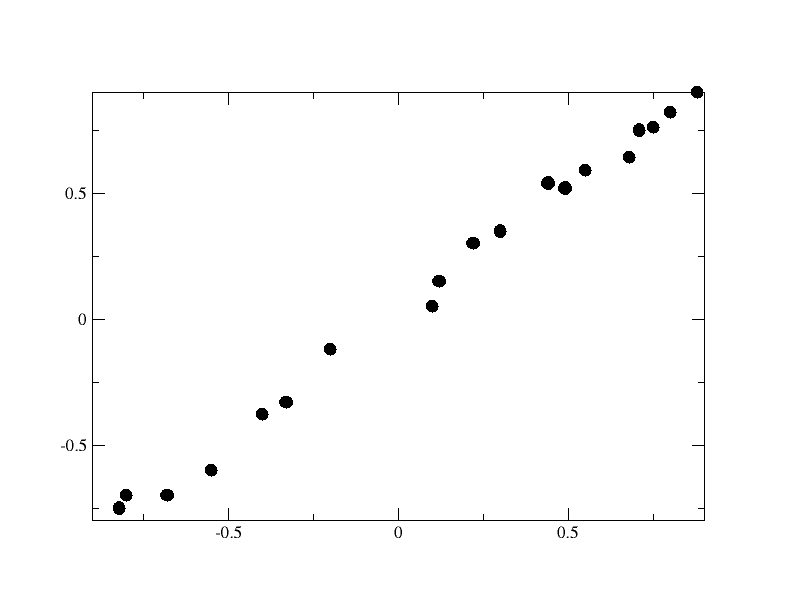
\includegraphics[scale =0.8]{pca.png}\\
\noindent The 45 degree rotation can be written as
\begin{align*}
	z_1 = \frac{\sqrt{2}}{2} (x_1 + x_2)\\
	z_2 = \frac{\sqrt{2}}{2} (x_1 - x_2)\\
\end{align*}
The above equation can be written in matrix form\\
\begin{align*}
\left( \begin{array} {c c}
z_1 & z_2 
\end{array} \right)
=\left( \begin{array} {c c}
z_1 & z_2 
\end{array} \right)
\left( \begin{array} {c c}
\frac{\sqrt{2}}{2}  & \frac{\sqrt{2}}{2} \\
\frac{\sqrt{2}}{2}  & -\frac{\sqrt{2}}{2} \\
\end{array} \right)\\
\end{align*}
\noindent We call $W_1 = (\frac{\sqrt{2}}{2}, \frac{\sqrt{2}}{2})^T$, and $W_2 = (\frac{\sqrt{2}}{2}, -\frac{\sqrt{2}}{2})^T$\\
In general, we can write the transform with W\\
\begin{align*}
\left( \begin{array} {c c}
z_1 & z_2 
\end{array} \right)
=\left( \begin{array} {c c}
x_1 & x_2 
\end{array} \right)
\left( \begin{array} {c c}
w_{11}  & w_{21} \\
w_{12}  & w_{22} \\
\end{array} \right)\\
\end{align*}
Writing Z and X in row vectors instead of column vector looks a little weird. The reason we do this is when we have multiple samples, we will increase number of rows to accommodate more samples.\\
{\bf Miltiple Sample representation and Algorithm Review}\\
If there are n samples, the transformation can be written in matrix notation\\
\begin{align*}
\left( \begin{array} {c c}
z_{11} & z_{12} \\
z_{21} & z_{22} \\
... & ... \\
z_{n1} & z_{n2} \\
\end{array} \right)
=\left( \begin{array} {c c}
x_{11} & x_{12} \\
x_{21} & x_{22} \\
... & ... \\
x_{m1} & x_{m2} \\
\end{array} \right)
\left( \begin{array} {c c}
w_{11}  & w_{21} \\
w_{12}  & w_{22} \\
\end{array} \right)\\
\end{align*}
In order to reduce to dimension, the goal is to find the transformation matrix W so that $(z_{11}, z_{21},...z_{n1})^T$ have the maximum variance. The dimension which has to maximum variance is the principle component. If we assume the data we have is processed and have mean at 0. Then the variance of Z is\\
\begin{align*}
	Z^T Z
=\left( \begin{array} {c}
W_{1}^T\\
W_{2}^T\\
\end{array} \right)\\
\left( \begin{array} {c c c c}
x_{11} & x_{21} &...& x_{m1} \\
x_{21} & x_{22} &...& x_{m2} \\
\end{array} \right)\\
\left( \begin{array} {c c}
x_{11} & x_{12} \\
x_{21} & x_{22} \\
... & ... \\
x_{m1} & x_{m2} \\
\end{array} \right)
\left( \begin{array} {c c}
W_{1}  & W_{2} \\
\end{array} \right)\\
= W^T X^T X W.
\end{align*}
Here we use some intuition to analyze the variance and leave the rigorous proof in next. By intuition we imagine $W_1$, $W_2$ ... $W_d$ be the eigenvectors of $X^TX$, namely
\begin{align*}
	X^TX W_k = \lambda_k W_k
\end{align*}
Then 
\begin{align*}
	W_k^T X^T X W_k = \lambda_k W_k^T W_k = \lambda_k
\end{align*}
Therefore, in order to maximize $W_k^T X^T X W_k$, $W_k$ has to be the corresponding eigenvector of the maximum eigenvalue $\lambda_{max}$.\\

\noindent{\bf c. Rigorous Proof}\\
Suppose we have a data set (X,y) where x is the feature variable. It is an mxn matrix where m is the data size, and n is the dimension of the features
\begin{align*}
\left( \begin{array} {c c c c} 
x_{11} & x_{12} & ... & x_{1n} \\
x_{21} & x_{22} & ... & x_{2n}\\
... & ... & ...& ...\\
x_{m1} & x_{m2} & ...& x_{mn}\\
\end{array} \right) \\
\end{align*}

We call the feature vector associated with the ith data x(i), we consider a coordinate transformation:\\
\begin{align*}
	

\left( \begin{array} {c c c c} 
z_{11} & z_{12} & ...& z_{1n}\\
z_{21} & z_{22} & ...& z_{2n}\\
... & ... & ... & ... \\
z_{m1} & z_{m2} & ...& z_{mn}\\
\end{array} \right)
=
\left( \begin{array} {c c c c} 
x_{11} & x_{12} & ...& x_{1n}\\
x_{21} & x_{22} & ...& x_{2n}\\
... & ... & ...&\\
x_{m1} & x_{m2} & ...& x_{mn}\\
\end{array} \right)
\left( \begin{array} {c c c c}
w_{11}$  & w_{21} &... & w_{n1}\\
w_{12}$  & w_{22} &... & w_{n2}\\
... & ...&  ...& ...\\
w_{1n}$  & w_{22} &... & w_{nn}\\
\end{array} \right)\\
\end{align*}
The goal is to reduce the dimension of the feature to d, still have a good representation of the data.
When Z has only d (d<n) dimension, then \\
\begin{align*}
 \left( \begin{array} {c c c c} 
z_{11} & z_{12} & ...& z_{1d}\\
z_{21} & z_{22} & ...& z_{2d}\\
... & ... & ... & ... \\
z_{m1} & z_{m2} & ...& z_{md}\\
\end{array} \right)
=
 \left( \begin{array} {c c c c} 
x_{11} & x_{12} & ...& x_{1n}\\
x_{21} & x_{22} & ...& x_{2n}\\
... & ... & ... & ... \\
x_{m1} & x_{m2} & ...& x_{mn}\\
\end{array} \right)

\left( \begin{array} {c c c c}
w_{11}  & w_{21} &... & w_{d1}\\
w_{12}  & w_{22} &... & w_{d2}\\
... & ...&  ...& ...\\
w_{1n}$  & w_{22} &... & w_{dn}\\
\end{array} \right)\\
\end{align*}
The problem is how to choose d dimensions out of n.
We define the error function as
\begin{align*}
 \sum_i ^{m}  || x_i - z_i||_2^2   
=|| X - W WT x||_2^2 \textrm{This is a little involved} \\
W = argmax || X - X W WT||22
  = argmax tr(WT X^TX W)\\
\end{align*}
Let $w_1$, $w_2$,��, $w_n$ be the column vectors of matrix W, then \\
\begin{align*}
    tr(WT X^TX W)\\
= w_1^T X^TX w_1 + w_2^T X^TX w_2 +�� + w_d^T X^TX w_d\\
= \sum w_i^T w_i \lamdba_i (\lambda_i \textrm { is the ith eigenvalues of } X^T X)\\
\end{align*}
If $w_i$ are the eigenvector corresponding to $\lambda_i$ 
Then the maximum value of the trace is achieved when we take $w_1$ to $w_d$ as the eigenvectors associated with the first d maximum eigenvalues.


\end{document}